%!TEX root = ../template.tex
%%%%%%%%%%%%%%%%%%%%%%%%%%%%%%%%%%%%%%%%%%%%%%%%%%%%%%%%%%%%%%%%%%%%
%% chapter3.tex
%% NOVA thesis document file
%%
%% Chapter with a short latex tutorial and examples
%%%%%%%%%%%%%%%%%%%%%%%%%%%%%%%%%%%%%%%%%%%%%%%%%%%%%%%%%%%%%%%%%%%%

\typeout{NT FILE chapter3.tex}				% se eu quiser mais um capitulo, tenho de copiar estas linhas
											% (da 1-9) -> e com as devidas alterações (ex.: chapter5, acknowledgements 2)

\chapter{Workflow Planning}\label{cha:III_workflow}

this is the best way
to write something

in LaTeX

% \begin{figure}[H]
% 	\centering
% 	
\includegraphics[height=1in]{snowman-bitmap}
% 	
\includegraphics[height=3in]{snowman-bitmap}
% 	
\includegraphics[height=6in]{snowman-bitmap}
% 	\caption{Imagem em formato \emph{bitmap} (JPG)}
% 	\label{fig:Figuras_Tree_silhouettes-bitmap}
% \end{figure}

this is the best way
to write something

in LaTeX

\begin{figure}[htbp]
	\centering
	
\includegraphics[height=1in]{snowman-bitmap}
	\hfill
	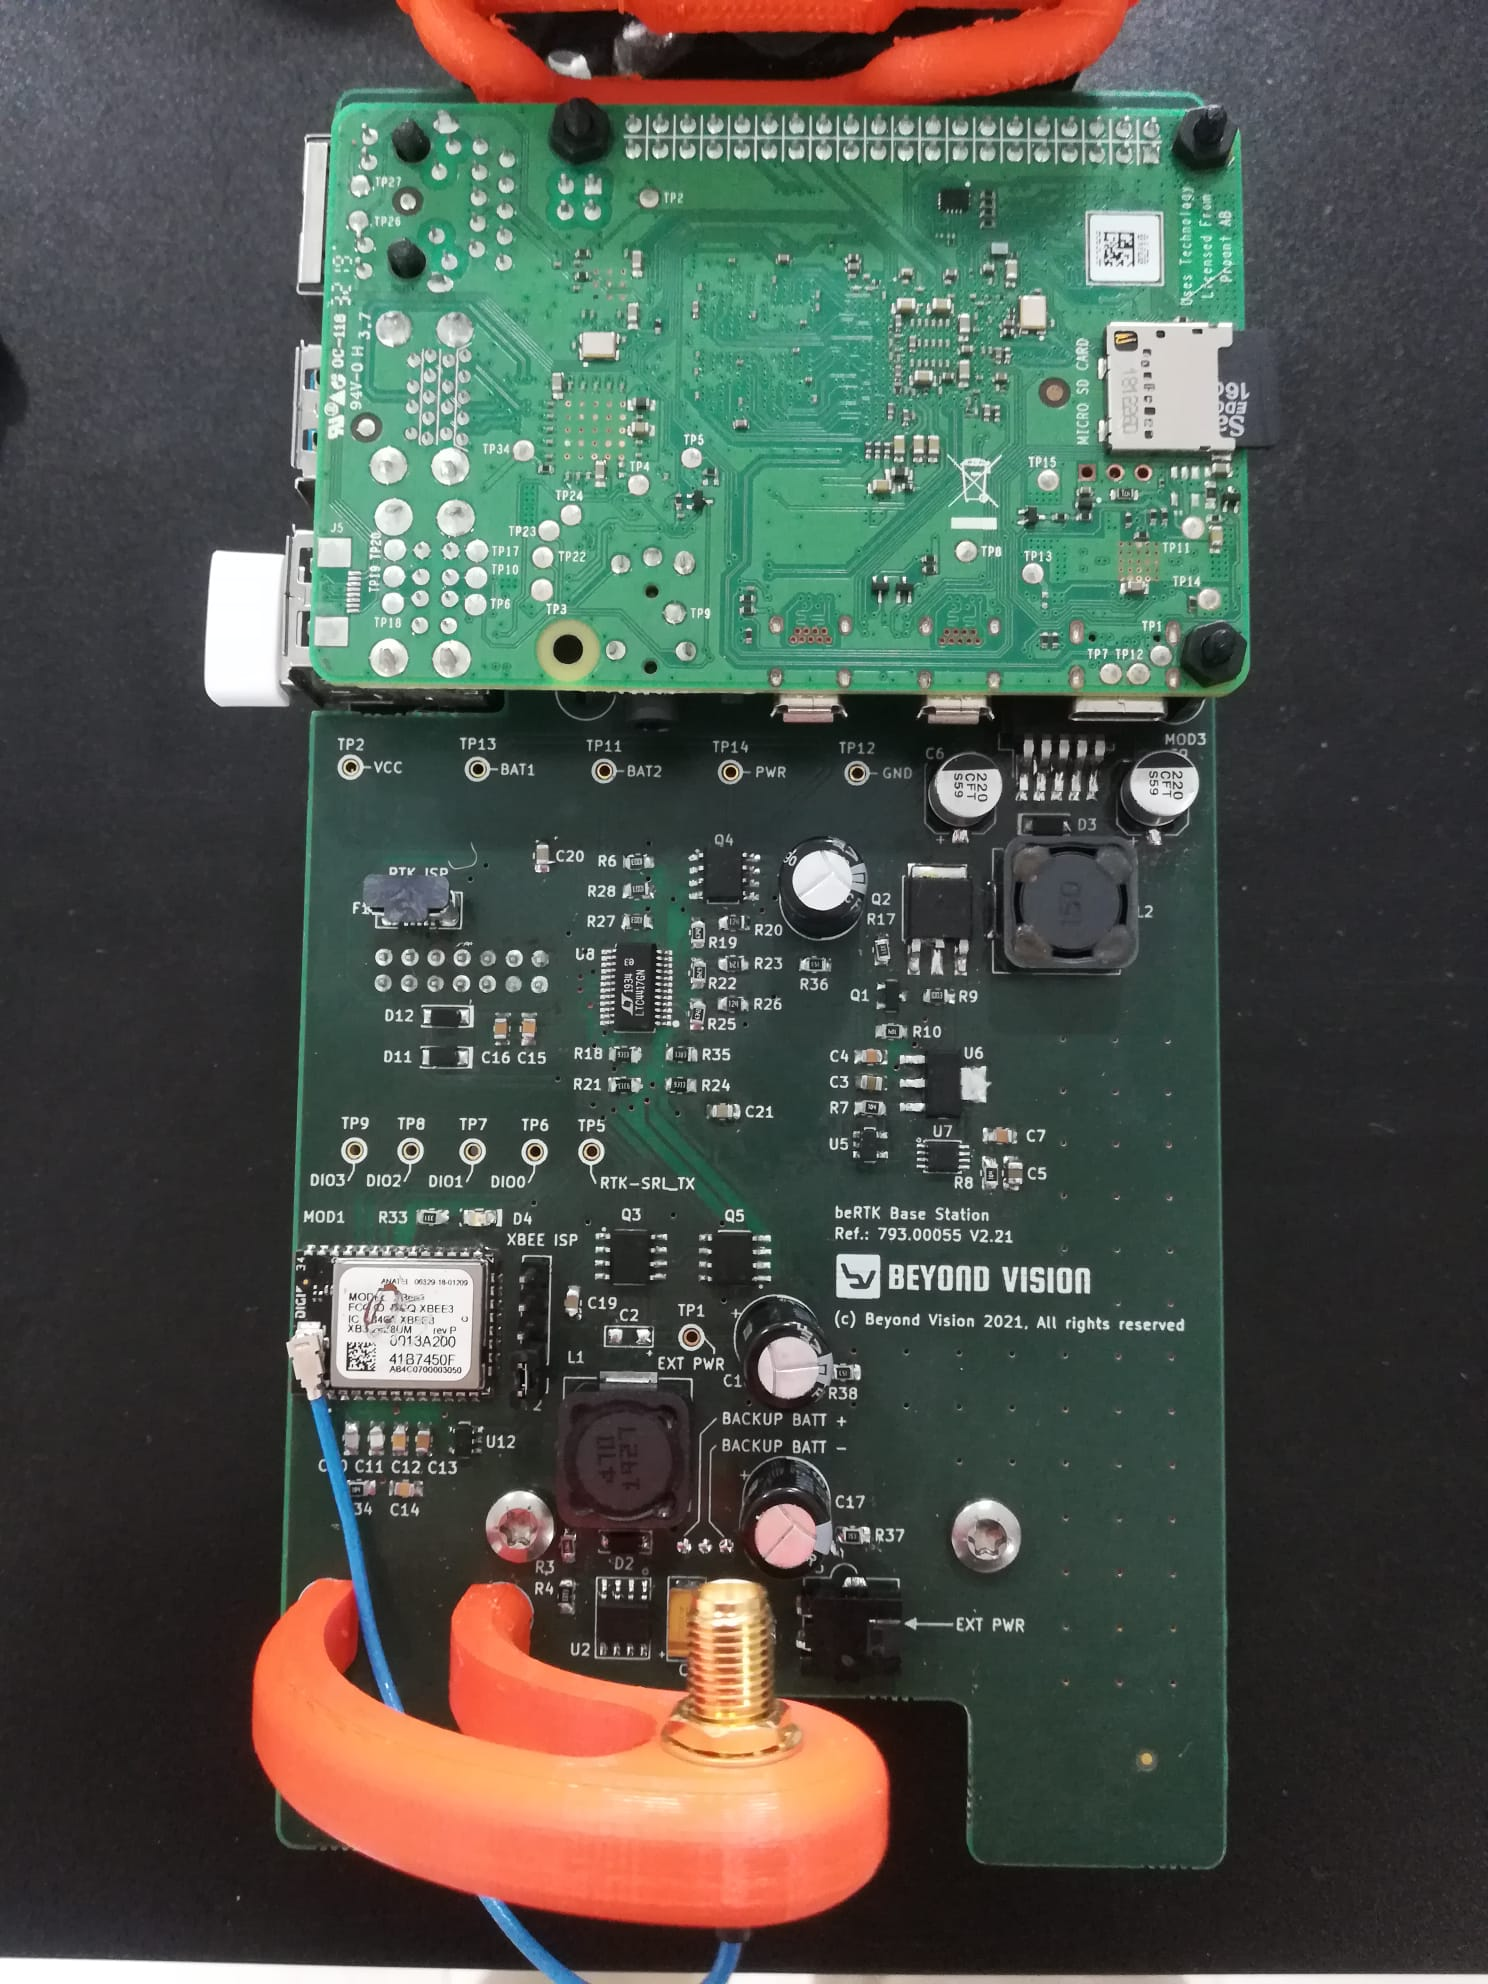
\includegraphics[height=2in]{Intro/old_BS}
	\caption{Imagem em formato \emph{bitmap} (JPG)}
	\label{fig:Figuras_Tree_silhouettes-bitmap}
\end{figure}

% Footnotes\footnote{This is a simple footnote.} will be numbered and shown in the bottom of the page.
 
% \begin{table}[ht]
% 	\caption{Test results summary.}
% 	\label{tab:hla:results}
% 	\centering
% 	\begin{tabular}{lccccc}
% 		\toprule
% 		\multicolumn{1}{c}{\textbf{Test}} & \textbf{Anomalies} & \textbf{Warnings} & \textbf{Correct} & \textbf{Categories} & \textbf{Missed}\\
% 		\midrule
% 		\cite{Beckman08}~Connection 	& 2 & 2	& 1	& \emph{C}				& 1 \\
% 		\cite{Artho03}~Coordinates'03 	& 1	& 4	& 1	& \emph{2B, 1C}			& 0 \\
% 		\cite{Artho03}~Local Variable	& 1	& 2	& 1	& \emph{A}				& 0 \\
% 		\cite{Artho03}~NASA				& 1	& 1	& 1	& ---					& 0 \\
% 		\cite{Artho04}~Coordinates'04	& 1	& 4	& 1	& \emph{3C}				& 0 \\
% 		\cite{Artho04}~Buffer			& 0	& 7	& 0	& \emph{2A, 1B, 2C, 2D}	& 0 \\
% 		\cite{Artho04}~Double-Check		& 0	& 2	& 0	& \emph{1A, 1B}			& 0 \\
% 		\cite{Flanagan04}~StringBuffer	& 1	& 0	& 0	& ---					& 1 \\
% 		\cite{Praun03}~Account			& 1	& 1	& 1	& ---					& 0 \\
% 		\cite{Praun03}~Jigsaw			& 1	& 2	& 1	& \emph{C}				& 0 \\
% 		\cite{Praun03}~Over-reporting	& 0	& 2	& 0	& \emph{1A, 1C}			& 0 \\
% 		\cite{Praun03}~Under-reporting	& 1	& 1	& 1	& ---					& 0 \\
% 		\cite{IBM-Rep}~Allocate Vector	& 1	& 2	& 1	& \emph{C}				& 0 \\
% 		Knight Moves					& 1	& 3	& 1	& \emph{2B}				& 0 \\
% 		\midrule
% 		\textbf{Total} & \textbf{12} & \textbf{33} 		& \textbf{10} 	& \textbf{5A, 6B, 10C, 2D}	& \textbf{2}\\
% 		\bottomrule
% 	\end{tabular}
% \end{table}
